
\documentclass{llncs}

\usepackage{epsfig}
\usepackage{graphicx}
\usepackage{color}
\usepackage{amsfonts}
\usepackage{amsmath}
\usepackage{mathabx}
%\usepackage{hyperref}
%\usepackage{subfigure}
%\usepackage[colorinlistoftodos, textwidth=3.2cm, shadow]{todonotes}

\usepackage{algorithm}
\usepackage{fixltx2e}
\usepackage{algpseudocode}
\usepackage{adjustbox}

\usepackage{multirow}

% To use Call inside another Call (algorithms)
\MakeRobust{\Call}


%%%%%%%%%%%%%%%%%%%%%%%%%%%%%%%%%%%%%%%%%%
%
% Title
%
%%%%%%%%%%%%%%%%%%%%%%%%%%%%%%%%%%%%%%%%%%
\title{StarCraft Bots and Competitions
%\thanks{Supported by ...}
}

\author{David~Churchill\inst{1} \and
		Mike~Preuss\inst{2}		
		Florian~Richoux\inst{3} \and
		Gabriel~Synnaeve\inst{4} \and
		Alberto~Uriarte\inst{5} \and
		Santiago~Onta\~{n}\'{o}n\inst{5} \and 
		}

\institute{
	Computing Science Department of the University of Alberta, Edmonton, Canada. \\
	\email{cdavid@cs.ualberta.ca}
\and
	Department of Computer Science of Technische Universit{\"a}t Dortmund, Germany.
	\email{mike.preuss@cs.tu-dortmund.de}
\and
	Nantes Atlantic Computer Science Laboratory (LINA) of the Universit{\'e} de Nantes, France. \\
	\email{florian.richoux@univ-nantes.fr}
\and
	Cognitive Science and Psycholinguistics (LSCP) of ENS Ulm, Paris, France. \\
	\email{gabriel.synnaeve@gmail.com}
\and
	Computer Science Department at Drexel University, Philadelphia, PA, USA. \\
	\email{\{santi,albertouri\}@cs.drexel.edu}
}

\begin{document}

\maketitle

\section{State of the Art Bots for StarCraft}\label{sec:bot}

Thanks to the recent organization of international game AI competitions focused around the popular StarCraft game (see Section \ref{sec:competition}), several groups have been working on integrating many of the techniques described in the previous section into complete ``bots'', capable of playing complete StarCraft games. In this section we will overview some of the currently available top bots.

%\subsection{RTS Bot Architectures}\label{sec:integration}

Playing an RTS game involves dealing with all the problems described above. A few approaches, like CAT \cite{LTW}, Darmok \cite{OntanonMSR10} or ALisp \cite{Marthi05} try to deal with the problem in a monolithic manner, by using a single AI technique. However, none of those systems aims at achieving near human performance. In order to achieve human-level performance, RTS AI designers use a lot of domain knowledge in order to divide the task of playing the game into a collection of sub-problems, which can be dealt-with using individual AI techniques.

\begin{figure}[h!]
  \begin{adjustbox}{addcode={\begin{minipage}{\width}}{\caption{%
    %\centering
            Architecture  of 7  StarCraft bots  obtained by  analyzing
            their  source code.  Modules  with  black background  sent
            commands  directly to  StarCraft, dashed  arrows represent
            data flow, and solid arrows represent control.
          }\end{minipage}},rotate=90,center}
    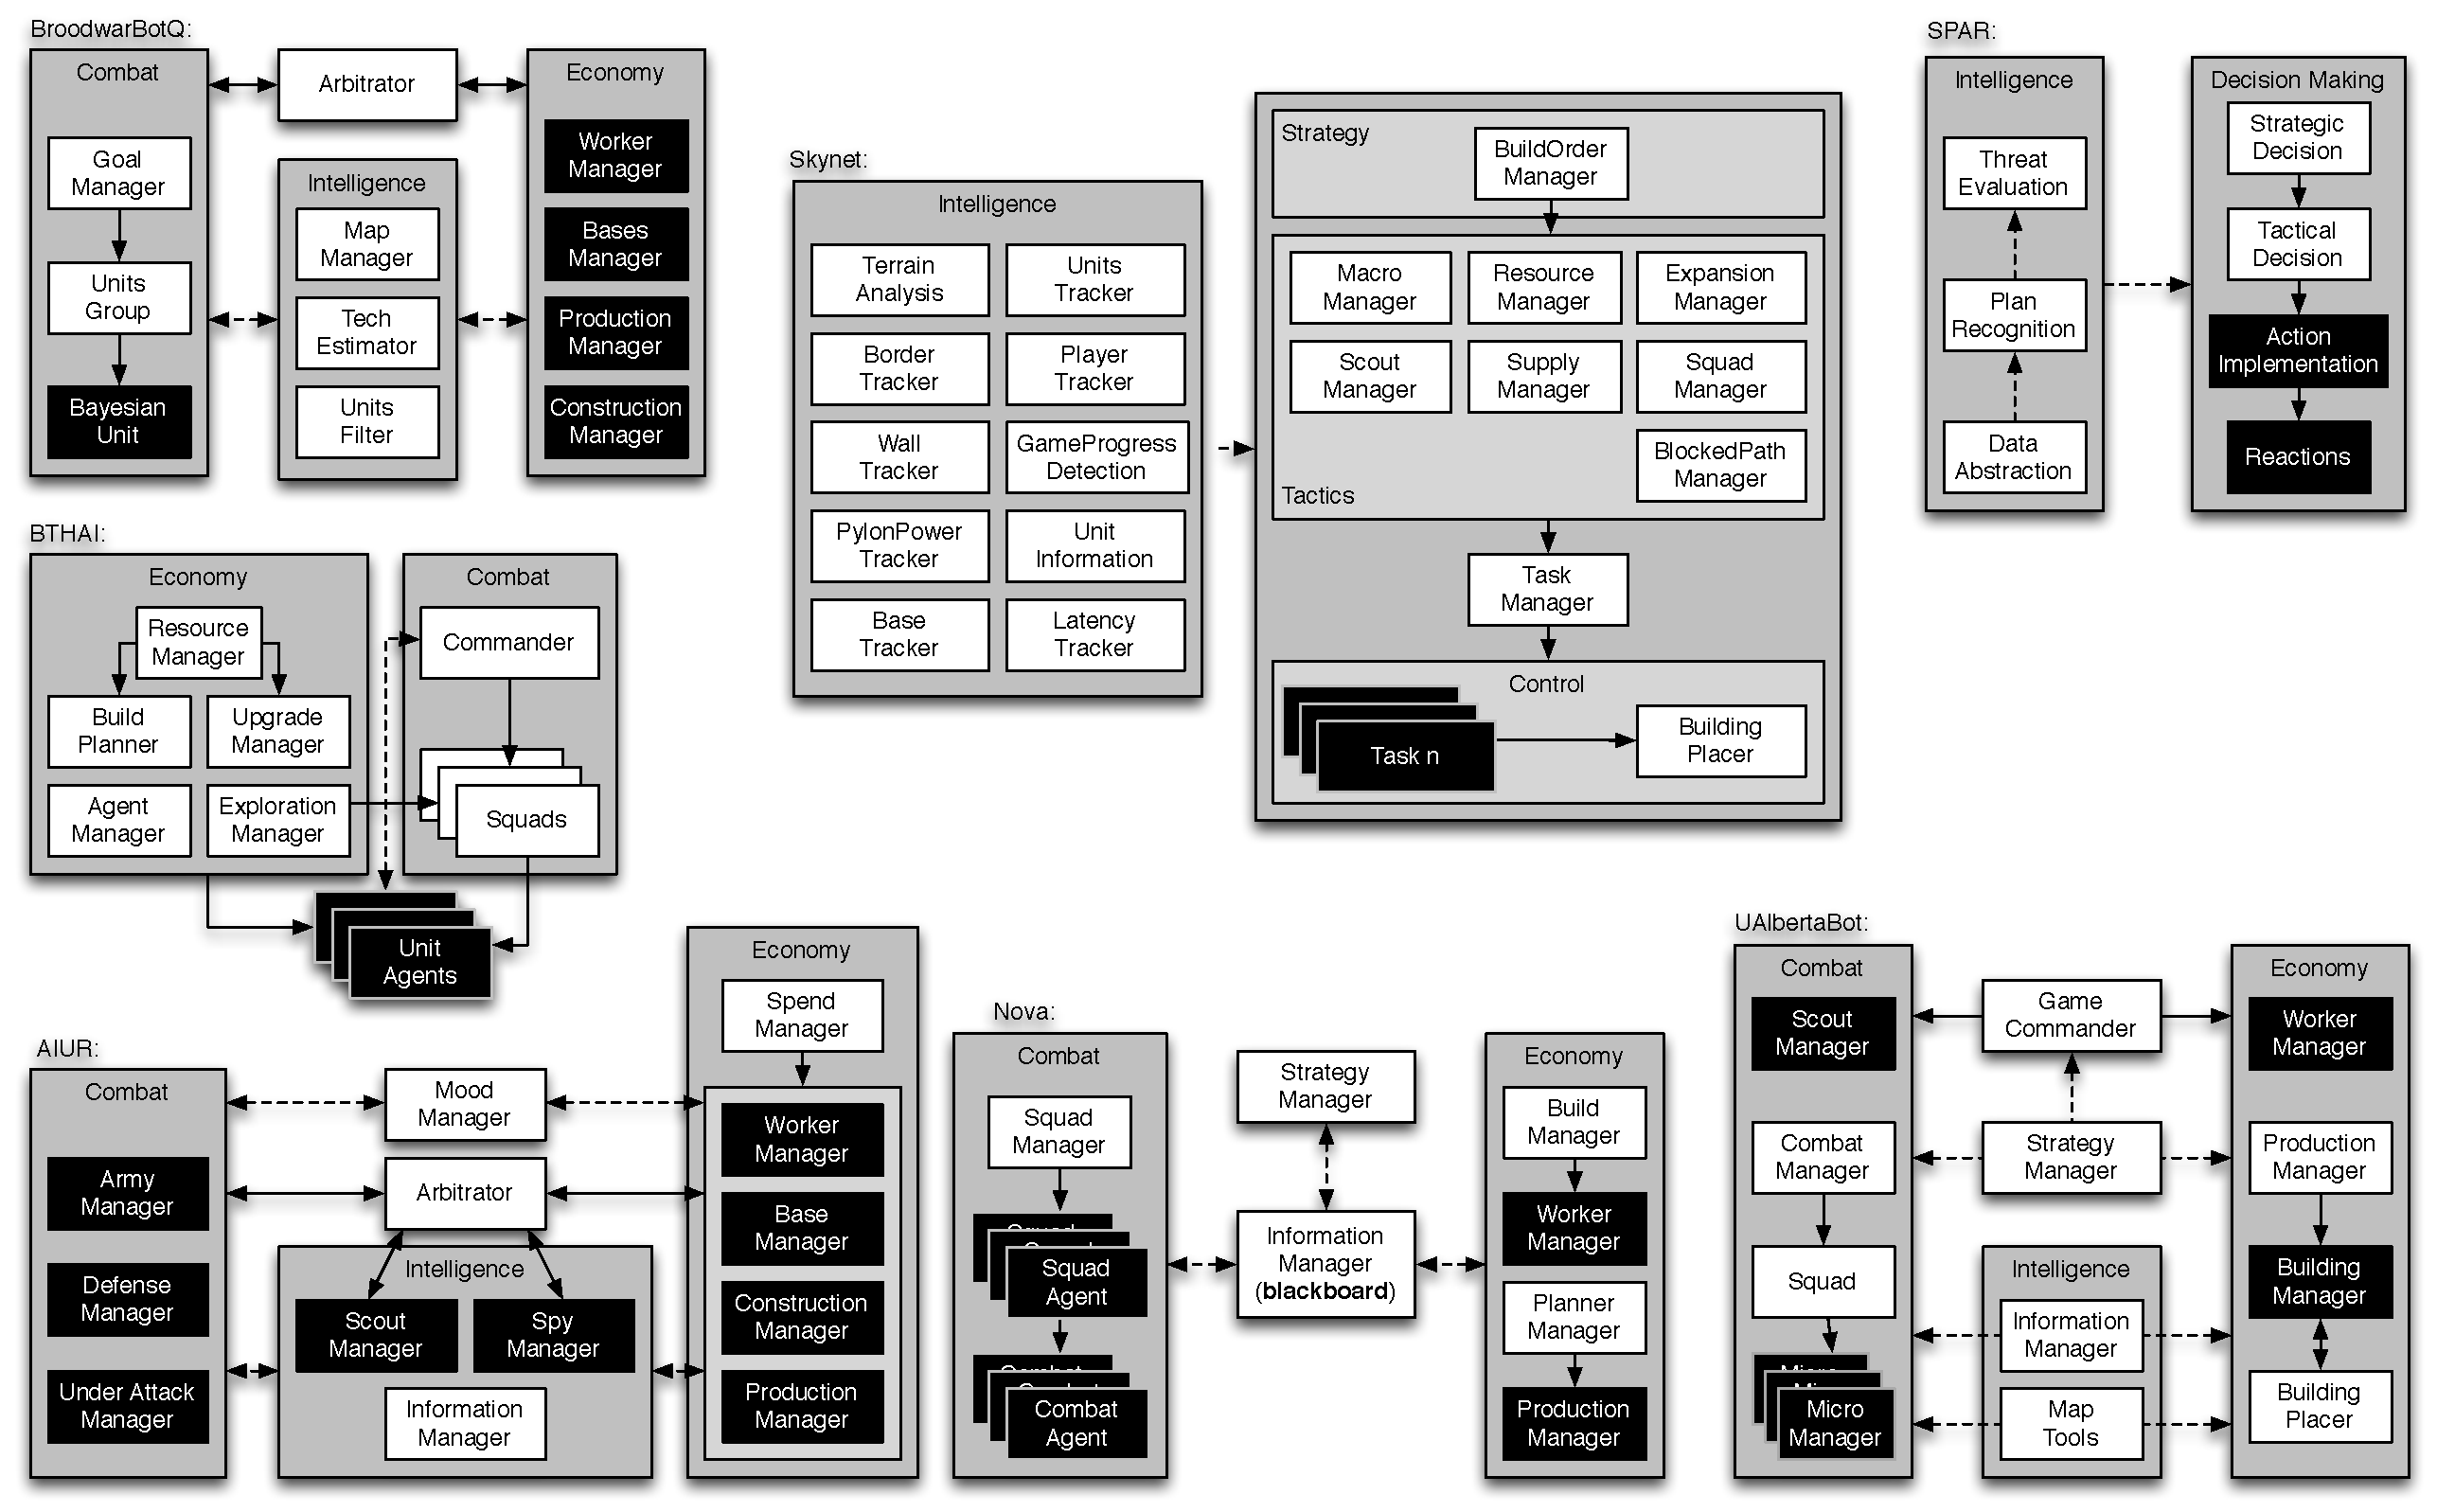
\includegraphics[width=0.935\textheight]{figures/figure-bot-architectures-wide.pdf}
    % \caption{Architecture of 7  StarCraft bots obtained by analyzing
    % their  source code.  Modules with  black background  sent commands
    % directly  to StarCraft,  dashed  arrows represent  data flow,  and
    % solid arrows represent control.}
  \end{adjustbox}
    \label{fig:bot-architecture}
\end{figure}

Figure \ref{fig:bot-architecture} shows some representative examples of the architectures used by different bots in the AIIDE and CIG StarCraft AI competitions (see Section \ref{sec:competition}): BroodwarBotQ \cite{SynnaeveMicroCig11}, Nova \cite{uriarte2012kiting}, UAlbertaBot \cite{churchill2011build}, Skynet, SPAR, AIUR, and BTHAI \cite{Hagelback12}. Each box represents an individual module with a clearly defined task (only modules with a black background can send actions directly to StarCraft). Dashed arrows represent data flow, and solid arrows represent control (when a module can command another module to perform some task). For example, we can see how SPAR is divided in two sets of modules: {\em intelligence} and {\em decision making}. Intelligence in SPAR has three modules dedicated to analyze the current situation of the game. Decision making in SPAR is done through four hierarchically organized modules, with the higher-level module ({\em strategic decision}) issuing commands to the next module ({\em tactical decision}), which sends commands to the next module ({\em action implementation}), and so on. Only the two lower-level modules can send actions directly to StarCraft. 

On the other hand, bots such as Nova or BroodwarBotQ (BBQ) only use a hierarchical organization for {\em combat} (controlling the attack units), but use a decentralized organization for the rest of the bot. In Nova and BBQ, there is a collection of modules that control different aspects of the game (workers, production, construction, etc.). These modules can all send actions directly to StarCraft. In Nova those modules coordinate mostly through writing data in a shared blackboard, and in BBQ they coordinate only when they have to use a shared resource (unit) by means of an arbitrator: a bidding market and broker for settling units control, military and civilian groups/task forces bid for units proportionally to their usefulness and the task importance.

By analyzing the structure of these bots, we can see that there are two main tools being used in these integration architectures:

\begin{itemize}
\item {\em Abstraction}: complex tasks can be formulated at different levels of abstraction. For example, playing an RTS game can be seen as issuing individual low-level actions to each of the units in the game, or at a higher level, it can be seen as deploying a specific strategy (e.g. a ``BBS strategy'', or a ``Reaver Drop'' strategy). Some bots, reason at multiple levels of abstraction at the same time, making the task of playing StarCraft simpler. Assuming that each module in the architecture of a bot has a goal and determines some actions to achieve that goal, the actions determined by higher-level modules are considered as the goals of the lower level modules. In this way, each module can focus on reasoning at only one level of abstraction, thus, making the problem easier.

\item {\em Divide-and-conquer}: playing a complex RTS, such as StarCraft, requires performing many conceptually different tasks, such as gathering resources, attacking, placing buildings, etc. Assuming each of these tasks can be performed relatively independently and without interference, we can have one module focusing on each of the tasks independently, thus making the problem easier. 
\end{itemize}

If we imagine the different tasks to perform in a complex RTS game in a two-dimensional plane, where the vertical axis represents abstraction, and the horizontal axis represents the different aspects of the game (combat, resource gathering, etc.), abstraction can be seen as dividing the space with horizontal lines, whereas divide-and-conquer divides the space using vertical lines.

Different bots use different combinations of these two tools. Looking back at Figure \ref{fig:bot-architecture}, we can see the following use of abstraction and divide-in-conquer in the bots:

\begin{itemize}
\item
  BroodwarBotQ\footnote{\url{http://github.com/SnippyHolloW/BroodwarBotQ}}:
  uses  abstraction for  {\em combat}, and  divide-and-conquer for
  {\em economy}  and  {\em intelligence  gathering}. To  avoid  conflicts
  between modules (since  the individual tasks of each  of the modules
  are not completely independent), BBQ uses an arbitrator.
\item  Nova\footnote{\url{http://nova.wolfwork.com/}}:  is similar  in
  design as  BroodwarBotQ, and uses  abstraction for {\em combat},
  and  divide-and-conquer for  {\em economy}.  The differences  are
  that Nova does not have  an arbitrator to resolve conflicts, but has
  a  higher-level   module  ({\em  strategy   manager}),  which  posts
  information to the blackboard that the rest of modules follow (thus,
  making use of abstraction).
\item
  UAlbertaBot\footnote{\url{http://github.com/davechurchill/ualbertabot/}}:
  also  uses abstraction  in  {\em combat} like  the previous  two
  bots. But it  also uses it in {\em economy}: as  can be seen, the
  production manager sends commands to the building manager, who is in
  charge   of   producing   the   buildings.  This   bot   also   uses
  divide-and-conquer, and  tasks like scouting  and resource gathering
  are managed by separate, independent modules.
\item       Skynet\footnote{\url{http://code.google.com/p/skynetbot/}}:
  makes     extensive     use      of     both     abstraction     and
  divide-and-conquer.  We  can see a  high level module  that issues commands  to a
  series of  tactics modules. The  collection of tactic  modules queue
  {\em  tasks} (that  are analogous  to the  abstract actions  used in
  SPAR).  Each different  task has  a specific  low level  module that
  knows how to  execute it. Thus, Skynet uses  a 3 layered abstraction
  hierarchy,  and uses  divide-and-conquer  in all  levels except  the
  highest.
\item
  SPAR\footnote{\url{http://www.planiart.usherbrooke.ca/projects/spar/}}:
  only uses abstraction. Its high-level module determines the strategy
  to  use,  and  the  tactical  decision  module  divides  it  into  a
  collection  of {\em  abstract  actions}, that  are  executed by  the
  lower-level modules.
\item  AIUR\footnote{\url{http://code.google.com/p/aiurproject/}}:  is
  mainly divide-and-conquer oriented,
  with a  slight abstraction on  {\em economy} due to a  SpendManager deciding
  how  to  spend  and  share  resources  among  Base,  Production  and
  Construction Managers.  At the beginning of a  game, the MoodManager
  initializes  a  ``mood''  which  will  influence  both  tactics  and
  strategy. {\em Combat} is divided into three  independent managers: the
  {\em  Defense Manager},  controlling  military units  when there  is
  nothing special, the {\em  Under Attack Manager}, activated when the
  opponent is attacking our bases,  and the {\em Army Manager}, taking
  control of units when it is time to attack, following a timing given
  by the  current mood. This bot  does not manage however  any kind of
  reactive controls so far.
\item  BTHAI\footnote{\url{http://code.google.com/p/bthai/}}:  uses  a
  two-tier  abstraction hierarchy,  where a  collection  of high-level
  modules command a collection of lower-level agents in charge of each
  of  the units.  At  the high-level,  BTHAI uses  divide-and-conquer,
  having   multiple  high-level  modules   issuing  commands   to  the
  lower-level units.
\end{itemize}

Additionally, except for BTHAI, all other agents use divide-and-conquer at a higher-level bot design and divide all the modules into two or three categories: {\em intelligence gathering} and {\em decision making} (sometimes divided into {\em combat} and {\em economy}).

Some bots  using divide-and-conquer, assume  that each of  the modules
can act independently  and that their actions can  be executed without
interference.  BBQ,  UAlbertaBot and  AIUR, however use  an arbitrator
({\em Game Commander'} in UAlbertaBot) that makes sure that modules do
not send contradictory orders to  the same unit.  However, very little
bots handle  the problem of  how to coordinate resource  usage amongst
modules, for  instance BTHAI uses a  first-come-first-serve policy for
spending resources,  the first module  that requests resources  is the
one that gets them. Nova and Skynet are exceptions, and implement some
rudimentary prioritization based on the high level strategy. Following
available  resources and  timing,  AIUR's {\em  Spend Manager}  orders
Base,  Production   and  Construction  Managers  what   they  have  to
build/produce. It also orders to start tech research and upgrades. The
idea here is not to let the different managers allocate the resources they want, but to do the opposite, that is: finding how the AI can
spend the available money.

One  interesting aspect  of the  seven bots  described above  is that,
while all  of them (except AIUR) are  reactive at the  lower level
(reactive  control), most  if not  all of  them, are  scripted  at the
highest level  of abstraction. BTHAI reads build  and squad formations
from  a  predefined  script,   Nova's  {\em  Strategy  Manager}  is  a
predefined finite-state machine,  BBQ's construction manager reads the
build  order from a  predefined script,  and Skynet's  {\em BuildOrder
  Manager} is basically a predefined script. Such scripts describe the
strategy  that the  bots will  use, however,  such strategy  is always
fixed.   One could see  this pre-scripting  as if  each bot  defined a
``high-level programming language''  to describe StarCraft strategies,
and   the   bots   themselves    are   just   interpreters   of   such
strategy.  Compared  to  current  approaches  for Chess  or  Go,  this
scripting  seems a  rigid and  inflexible,  but responds  to the  much
higher complexity of the  StarCraft game.  An interesting exception to
that  is  UAlbertaBot, which  uses  a  search  algorithm in  the  {\em
  Production  Manager}  to find  near-optimal  build orders.   Another
interesting case is  AIUR, that uses a {\em  Mood Manager} to randomly
pick  a mood among  six (cheese,  rush, aggressive,  defensive, macro,
fast  expand), which  will  influence the  build  order, strategy  and
tactics. % All of  them  scripted so  far,  but build  orders can  been modified but  the Spend Manager, following  available resources.  This mood can change during the game, regarding the opponent behavior.

In conclusion, we can see that there are two basic tools that can be used in an integration architecture: abstraction and divide-and-conquer, which are widely used by the existing StarCraft bots. For space reasons, we do not include an exhaustive comparison of the architectures of all the participating bots. Some other bots have been documented by their authors, such as SCAIL \cite{YoungSCAIL} or QUORUM \cite{young2012evolutionary}.
%This section has focused on discussing the architecture of existing StarCraft bots. 
Let us now focus on their performance.

%\subsection{Individual AI Techniques}\label{sec:techniques}

%{\color{red} TODO}

\section{Recent StarCraft AI Competitions}\label{sec:competition}

This section reviews the results of the recent international competitions on AI for StarCraft. These competitions, typically co-located with scientific conferences, have been possible thanks to the existence of the Brood War Application Programming Interface 
(BWAPI)\footnote{\url{http://code.google.com/p/bwapi/}}, which 
enables replacing the human player interface with C++ code.
%A consequence of this indirect way of integrating new bots is that every machine can only run one custom bot, requiring two computers for a 2-player game.
The following subsections summarize the results of all the StarCraft AI competitions held at the AIIDE (Artificial Intelligence for Interactive Digital Entertainment) and CIG (Computational Intelligence in Games) conferences during the past years. Since 2011, the CIG and AIIDE competitions have typically been held in August / September in each year, as the conferences are scheduled quite close to each other. As a consequence of this, many of the same bots get entered into both competitions.

Additionally we analyze the statistics from the StarCraft Bot Ladder, where the best bots play against each other continuously over time. 

\subsection{AIIDE}\label{sec:AIIDE}

\subsubsection{AIIDE 2010}

Started in 2010, the AIIDE StarCraft AI Competition\footnote{\url{http://www.StarCraftAICompetition.com}} is the most
well known and longest running StarCraft AI Competition in the world. Each year,
AI bots are submitted by competitors to do battle within the retail version of
StarCraft: Brood War, with prizes supplied by Blizzard Entertainment. %This competition has been made possible by the BWAPI StarCraft programming interface, which allows players to write programs which can retrieve game data and issue game commands to StarCraft via an easy to use C++ API.


The first competition in 2010 was organized and run by Ben Weber in the Expressive
Intelligence Studio at University of California, Santa Cruz\footnote{\url{http://eis.ucsc.edu/StarCraftAICompetition}}. 26 total submissions
were received from around the world. As this was the first year of the competition,
and little infrastructure had been created, each game of the tournament was run 
manually on two laptop computers and monitored by hand to record the results. Also,
no persistent data was kept for bots to learn about opponents between matches.

The 2010 competition had 4 different tournament categories in which to compete. Tournament 1
was a flat-terrain unit micro-management battle consisting of four separate unit
composition games. Of the six competitors, FreSCBot won the competition with
Sherbrooke coming in 2nd place. Tournament 2 was another micro-focused game with
non-trivial terrain. Two competitors submitted for this category, with FreSCBot
once again coming in 1st by beating Sherbrooke.

Tournament 3 was a tech-limited StarCraft game on a single known map with no fog-of-war enforced. Players
were only allowed to choose the Protoss race, with no late game units allowed. 8 bots
faced off in this double-elimination tournament with MimicBot taking first place over Botnik in the final.
As this was a perfect information variant of StarCraft, MimicBot adopted a strategy of
``mimic its opponent's build order, gaining an economic advantage whenever possible'' which
worked quite well.

Tournament 4 was the complete game of {\em StarCraft: Brood War} with fog-of-war enforced. The tournament
was run with a random pairing double-elimination format with each match being best of 5 games.
Competitors could play as any of the three races, with the only limitations in gameplay
being those that were considered ``cheating'' in the StarCraft community. A map pool of
5 well-known professional maps were announced to competitors in advance, with a random map being chosen for each game.

Results are shown in Table \ref{tab:aiide2010}. The team that won was Overmind\footnote{\url{http://overmind.cs.berkeley.edu}}, from University of California, Berkeley. Using the Zerg race, their
strategy was to defend early aggression with zergling units while amassing mutalisk units,
which they used to contain and eventually defeat their opponents. The mutalisk is a very fast and agile
flying unit which is able to attack while moving with no drawback, which makes them quite a powerful
unit when controlled by a computer. Overmind used a potential-field
based micro-management system to guide their mutalisks, which led them to victory. Krasi0 came in 2nd place
with a standard defensive Terran opening strategy that transitioned into ``mech'' play in the late game.

\begin{table}[!t]
\caption{Ranking of the three best bots of the AIIDE 2010 competition}
\label{tab:aiide2010}
\centering
\begin{tabular}{|c|l|}
\hline
{\bfseries Rank} & {\bfseries Bot}\\
\hline
1 & Overmind \\
2 & Krasi0 \\
3 & Chronos \\
\hline
\end{tabular}
\end{table}

\subsubsection{AIIDE 2011}

In 2011 the University of Alberta hosted the competition, with organization by Michael Buro and
David Churchill\footnote{\url{https://skatgame.net/mburo/sc2011/}}. Due to a lack of entrants in tournament categories 1-3 in the 2010 competition, it was
decided that only the full game category would be played in the 2011 competition. Another important
change in the 2011 competition was the introduction of automated tournament-managing software running
StarCraft games simultaneously on 20 computers, allowing a total of 1170 games to be played in the five days that the tournament ran. 
This increase in games played also allowed the tournament
to switch to a round-robin format, eliminating the ``luck'' factor of the pairings inherent in bracket
style tournaments. The bot that achieved the highest win percentage over the course of the competition would
be determined the winner. Also, the competition became open-source, in an effort 
to prevent possible cheating and to promote healthy competition in future tournaments by giving
newcomers and easier entry point by basing their design off of previous bots.

In the  end, Skynet  won the competition  with its solid  Protoss play
(results  are  summarized   in  Table  \ref{tab:aiide2011}).  The  bot
executed one of a small set of strategies randomly at the start of the
match based on the map and the race of the opponent. Skynet would then
amass a  medium to large  sized army and  expand before moving  out to
attack. Good  use of Dragoon (powerful ranged ground unit with clumsy movement) range and  kiting micro-management allowed
it to hold off the early aggression of other bots such as UAlbertaBot,
which came in 2nd.

\begin{table}[!b]
\caption{Results of the five best bots of the AIIDE 2011 competition}
\label{tab:aiide2011}
\centering
\begin{tabular}{|c|c|c|}
\hline
{\bfseries Rank} & {\bfseries Bot} & {\bfseries Win \%} \\
\hline
1 & Skynet & 88.9\% \\
2 & UAlbertaBot & 79.4\% \\
3 & AIUR & 70.3\% \\
4 & ItayUndermind & 65.8\% \\
5 & EISBot & 60.6\% \\
\hline
\end{tabular}
\end{table}

UAlbertaBot used an early zealot-rush strategy to take advantage of the power of early game Protoss units. 
It would send out the first zealots that were made and immediately attack the enemy base, using a unit
counting heuristic to determine whether or retreat or keep pushing. Of note is that UAlbertaBot used an
online planning algorithm to construct all of its economic build-orders\cite{churchill2011build}, as no hard-coded build orders
were used. 

AIUR also chose  Protoss, with a strategy that was in between Skynet
and UAlbertaBot in terms of  attack timings.  At that time, AIUR chose
one  mood among  five (leading  to slightly  different  strategies and
tactics) at the  beginning of a game and kept it  until the end. These
five moods were: 1. Rush: the bot tries early attacks, and have good
  probabilities to send the two or three first Zealots (basic contact attack ground unit) to harass the
  opponent. 2. Aggressive: it has less chance to perform harasses with
  the first Zealots, and the first attack is usually a bit delayed
  with regard to the Rush mood. 3. Macro: the AI do not try any early attacks and focus a bit
  more on its economy before attacking. 4. Defense: AIUR  ``turtles'' and wait to have a consequent
  army before running an attack. 5. Fast expand:  the  first building  constructed it  a base
  expansion, for a very economical-oriented game. Notice that build orders are not fully hard-coded since they can be
altered by AIUR's Spend Manager.

Of  note  in  these  results  was that  a  rock-paper-scissors  effect
happened among  the top  3 finishers.  Of  the 30 rounds,  Skynet beat
UAlbertaBot 26  times, UAlbertaBot beat  AIUR 29 times, and  AIUR beat
Skynet  19 times.   Another notable  result is  that Overmind  did not
choose  to compete despite  winning the  2010 competition.   After the
competition,  many  bot  programmers  (including  the  Overmind  team)
realized that their  2010 strategy was quite easily  defeated by early
game rushing strategies,  and so they submitted a  Terran bot instead,
called Undermind, which finished in 7th.

% After the competition was over, a man vs. machine match was held between the winner (Skynet) and an
% ex-professional StarCraft player named Oriol Vinyals. Oriol was a competitor in the 2001 World Cyber
% Games StarCraft competition, and though he had been out of practice for a few years was still quite a
% good player. The match was arranged to see how well StarCraft AI bots had progressed and to see if
% they could actually beat a decent human opponent. 

\begin{figure}[t!]
    \centering
    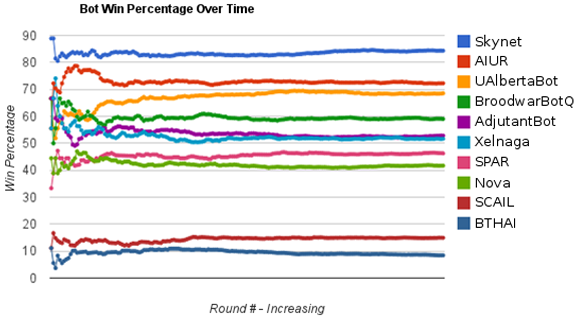
\includegraphics[width=\columnwidth]{figures/aiide2012_v2}
    \caption{Evolution of the win percentage of each bot participating in the AIIDE 2012 competition}
    \label{fig:aiide2012}
\end{figure}



% For the best-of-three match, Oriol chose his races randomly and ended up beating Skynet in a 2-0. 
% In the first match, Oriol played Zerg vs. Skynet's Protoss on Python, a four player map. Oriol chose
% to start with a fast expansion strategy and transition into two base mutalisk production. Skynet chose
% to rush with a few early zealots, which was luckily the best possible choice given Oriol's strategy.
% Skynet's initial attack destroyed Oriol's early defenses, and nearly won the game in the first few
% minutes, however it then proceeded to send zealots to attack one at a time rather than group up its
% units before moving in, which allowed Oriol to catch up. Once Oriol produced his mutalisks, Skynet did
% not produce sufficient air defenses and Oriol quickly destroyed Skynet's base. In the second game,
% Oril played Terran, again on Python. After holding off early Dragoon pressure from Skynet, Oriol
% moved out with a few marines, medics and tanks. Skynet tried to defend with its army of Dragoons,
% however due to poor unit targeting decisions it started to attack useless medics after the marines
% had died, rather than the tanks. Oriol overcame the Dragoon army and was victorious. Later analysis
% of the match concluded that Skynet, while dominant over the other bots, was unable to properly
% adapt and transition into a mid-game strategy in game one once its early pressure failed, and in game
% two made a key blunder in unit targeting which cost it the game. Humans were still in command.

\subsubsection{AIIDE 2012}

\begin{table}[!t]
\caption{Results of the five best bots of the AIIDE 2012 competition}
\label{tab:aiide2012}
\centering
\begin{tabular}{|c|c|c|}
\hline
{\bfseries Rank} & {\bfseries Bot} & {\bfseries Win \%} \\
\hline
1 & Skynet & 84.4\% \\
2 & AIUR & 72.2\% \\
3 & UAlbertaBot & 68.6\% \\
4 & BroodwarBotQ & 59.1\% \\
5 & AdjutantBot & 52.8\% \\
\hline
\end{tabular}
\end{table}

The University of Alberta also hosted the 2012 competition, with the major difference from the 2011
competition being the addition of file reading and writing for learning. Bots could now write information to disk during a
match, and then read the information during other matches, allowing them to adjust strategies based
on previous results. 6 of the 10 entrants used this feature to aid in strategy selection, including the
top 4 finishers. More improvements to the tournament environment also meant that a total of 4240 games
could now be played in the same time period. Results are shown in Table \ref{tab:aiide2012}.

Skynet once  again won  the competition with  its solid  Protoss build
orders  and  good  Dragoon  kiting.   AIUR  and  UAlbertaBot  switched
positions from  the previous  year to come  2nd and  3rd respectively.
Both  AIUR  and UAlbertaBot  used  data  stored  from the  results  of
previous games  to select a strategy for  future matches.  UAlbertaBot
did  this  using  the  UCB  \cite{auer2002finite} algorithm,  while  AIUR  used  a  uniform
distribution  to choose  its  mood before  altering this  distribution
after  some  games  against  the  same  opponent  to  favor  efficient
strategies, achieving  similar results than  UAlbertaBot. Notice that,
compared  to AIIDE 2011,  AIUR proposes  a new  mood, \textit{Cheese},
implementing a  Photon Cannon rush  strategy in order to  surprise the
opponent and  to finish the game  as soon as possible.   The effect of
this strategy selection process can be seen Figure \ref{fig:aiide2012}
which shows bot  win percentages over time.  While  the earlier rounds
of the tournament fluctuated wildly in results, eventually the results
converged to their  final values. One of the main  reasons for this is
due to  the bots  learning which strategies  to use as  the tournament
progressed.

\subsubsection{AIIDE 2013}

A total of 8 bots competed in the 2013 AIIDE competition with many of the same names from the 2012 competition, and some key updates were made to existing bots for 2013 which shook up the results from the previous years. UAlbertaBot took 1st place with a dominant 84.49\% win rate, with Skynet in 2nd with 72.77\%. The major addition to UAlbertaBot was a combat simulation package called SparCraft. UAlbertaBot was re-engineered so that it now always attacked from the first combat unit created, using the SparCraft system to simulate whether or not the bot could a fight against known enemy units, retreating automatically if it thought it could not. This addition, combined with some additional bug fixes led to the victory. Skynet and Aiur both implemented strategy learning in 2013, which is evident from \ref{fig:aiide2013} in which both Skynet and Aiur's win percentage over time climb dramatically from the first few rounds of the tournament to the later rounds. Ximp unfortunately crashed all games on the Fortress map and lost 10\% of its games for free as a result, which meant it could have possibly came in 2nd place if not for all those crashes. 

\begin{table}[!t]
\caption{Results of the five best bots of the AIIDE 2013 competition}
\label{tab:aiide2013}
\centering
\begin{tabular}{|c|c|c|}
\hline
{\bfseries Rank} & {\bfseries Bot} & {\bfseries Win \%} \\
\hline
1 & UAlbertaBot & 84.49\% \\
2 & Skynet & 72.77\% \\
3 & AIUR & 58.51\% \\
4 & Ximp & 56.57\% \\
5 & ICEStarCraft & 48.53\% \\
\hline
\end{tabular}
\end{table}

\begin{figure}[t!]
    \centering
    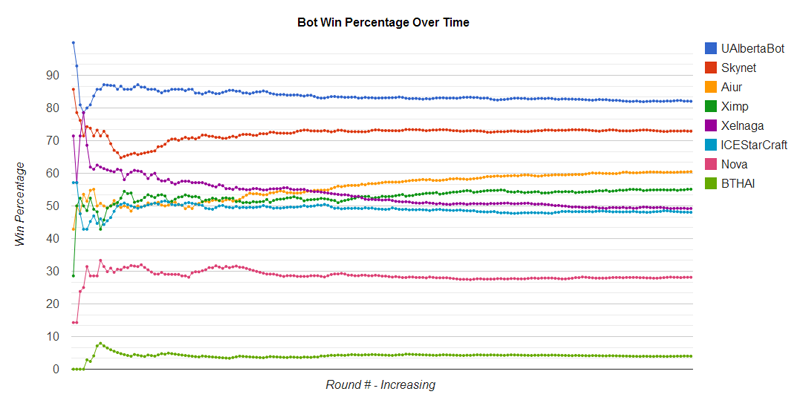
\includegraphics[width=\columnwidth]{figures/aiide2013}
    \caption{Evolution of the win percentage of each bot participating in the AIIDE 2013 competition}
    \label{fig:aiide2013}
\end{figure}

\subsubsection{AIIDE 2014}

The 2014 AIIDE competition saw 18 total entrants, over double the number from the 2013 competition. This dramatic increase in numbers was partially because of a large advertising effort by competition organizers, combined with the inclusion of all the 2013 competition entrants (if they had not re-submitted new versions). UAlbertaBot and Skynet who finished 1st and 2nd the year before were not updated in 2014 and so their previous versions were re-submitted. Along with the larger registration numbers came a lot of new Terran bots, a welcome change from the Protoss-dominated fields of previous years. The tournament managing software also underwent some major updates in 2014, allowing for faster game scheduling and the easy pausing and resuming of tournaments, resulting in 10251 total games being played, which was almost double the amount of 5579 from the previous year.

The results of the 2014 competition were dramatically different from previous years. Since 2011 the top 3 bots in the AIIDE competition had been some permutation of Skynet, UAlbertaBot, and Aiur, and in 2014 the top 3 finishers were all completely different. In first place was IceBot with a win rate of 85.85\%, which had a complete overhaul in terms of strategy and tactics from the previous year. IceBot had several strategies which it could implement, most starting with an early bunker defense and transitioning into attacking once a set of heuristics conditions had been met. IceBot's source code was originally based on Aiur's modular design, and changed to play the Terran race. In a close 2nd place finish was Ximp - which had fixed the crashes and logic errors which had plagued it the year before. Ximp implemented a solid forge-first fast expansion strategy which transitioned into late-game carrier play. By building a large amount of early photon cannons in its expansion, Ximp was easily able to stop most of the early rushing bots, and then holding them off until its carriers cleaned up in the late game. 3rd place was taken by LetaBot, a new Terran bot whose source code was written on top of the 2012 version of UAlbertaBot and changed to play the Terran race. LetaBot implemented a number of strategies including a 'cheesy' but strong bunker rush strategy which killed many bots very quickly, as well as a Wraith (mid-game flying unit) strategy. 

\begin{table}[!t]
\caption{Results of the five best bots of the AIIDE 2014 competition}
\label{tab:aiide2014}
\centering
\begin{tabular}{|c|c|c|}
\hline
{\bfseries Rank} & {\bfseries Bot} & {\bfseries Win \%} \\
\hline
1 & ICEBot & 85.86\% \\
2 & Ximp & 84.64\% \\
3 & LetaBot & 82.09\% \\
4 & AIUR & 70.94\% \\
5 & Skynet & 68.74\% \\
\hline
\end{tabular}
\end{table}

\subsubsection{AIIDE 2015}

The 2015 AIIDE competition was the largest competition to date with 23 total bots competing. The competition environment was also changed so that the tournament was now run on virtual machines instea dof physical machines. Doing this enabled the tournament to run for a full two weeks instead of the normal one week, resulting in a total of 20788 games being played - 90 full round robins between each bot pairing. 2015 saw the most even distribution of race selection ever in a Starcraft AI competition, with 5 new Zerg submissions along with 7 Protoss bots and 9 Terran bots. The first ever Random race entry was also submitted as UAlbertaBot had been updated to play all three of the available races. When playing Random race, Starcraft randomly assigns one of Protoss, Terran, or Zerg after the game has started, with your opponent not knowing which race you are until they have scouted you on the map. This provides a significant advantage as the enemy's initial build order must now have a period of uncertainty during which is has to guess what race it is playing against.

The results of the 2015 competition were extremely close, with 1st / 2nd place as well as 3rd / 4th place being separated by less than 1\% win rate. 1st place was won by Tscmoo, a new Zerg bot which played nearly a dozen different strategies, learning which one to choose over time via the file I/O system. In a close second place was ZZZKbot, which implement a 4-pool Zergling rush strategy every game. Despite the relatively simple strategy, most bots did not have proper defense capabilities and lost in very short games. In 3rd place was Overkill, another Zerg bot which had several different strategies including Mutalisks and Hydralisks, which learned over time as well. In a close 4th place was UAlbertaBot, which played Random and implemented three main rushing strategies - one for each race. An interesting result from this tournament was that despite UAlbertaBot coming 4th place, it finished with a winning rate greater than 50\% vs each other bot. Aiur came in 5th place and was a clear demonstration of how learning over time can dramatically improve results in a tournament, going from 63\% win rate early in the competition to a final win rate of over 73\%.

\begin{table}[!t]
\caption{Results of the five best bots of the AIIDE 2015 competition}
\label{tab:aiide2014}
\centering
\begin{tabular}{|c|c|c|}
\hline
{\bfseries Rank} & {\bfseries Bot} & {\bfseries Win \%} \\
\hline
1 & Tscmoo & 88.52\% \\
2 & ZZZKBot & 87.84\% \\
3 & Overkill & 80.69\% \\
4 & UAlbertaBot & 80.20\% \\
5 & Aiur & 73.02\% \\
\hline
\end{tabular}
\end{table}

% The 2012 man vs. machine match again used the winner of the competition (Skynet), who played against
% Mike Lange, also known as Bakuryu. At the time of the match, Bakuryu was an A- ranked Zerg player on ICCup,
% and known as one of the best non-Korean Zerg players in the world. Bakuryu was considered much
% stronger than Oriol at the time that the match was played, and the results showed that this was true.
% In the first game of the best-of-three, Bakuryu made Skynet look quite silly by running around inside
% Skynet's base with a small number of zerglings while Skynet's zealots and half of its worked chased
% then in vain. After killing off several probes and buying enough time to set up his expansion, he
% cleaned up Skynet's army with a flying army of mutalisks. In the second game, Bakuryu contained Skynet
% inside its base with a group of zerglings positioned within Skynet's expansion. Skynet then constructed
% several Dark Templar and along with some Dragoons and Zealots attacked into Bakuryu's expansion which
% was heavily defended, and was crushed almost instantly, allowing Bakuryu's zergling force to finish
% off the Protoss base. 

% In this match it was shown that the true weakness of state of the art StarCraft AI systems was that
% humans are very adept at recognizing scripted behaviors and exploiting them to the fullest. A human
% player in Skynet's position in the first game would have realized he was being taken advantage of and
% adapted his strategy accordingly, however the inability to put the local context (Bakuryu kiting his
% units around his base) into the larger context of the game (that this would delay Skynet until
% reinforcements arrived) and then the lack of strategy change to fix the situation led to an easy
% victory for the human. These problems remain as some of the main challenges in RTS AI today: to both recognize
% the strategy and intent of an opponent's actions, and how to effectively adapt your own strategy to 
% overcome them.

% All results, videos, and replays from the AIIDE StarCraft AI Competition can be found in \url{http://www.StarCraftAICompetition.com}.
% \footnote{\url{http://www.StarCraftAICompetition.com}}.

\begin{table*}[!t]
\caption{Results of the first round at CIG 2011, held in two brackets.
Qualified for the final round: UAlbertaBot and Skynet (from A), Xelnaga
and BroodwarBotQ (from B, the latter by comparing direct encounters
with BTHAI of which 6:4 were won)}
\label{tab:cig-first-round}
\centering
% bracket A
\begin{tabular}{|c|c|c|c|c|}
\hline
\multicolumn{5}{|c|}{Bracket A} \\ \hline
{\bfseries Rank} & {\bfseries Crashes} & {\bfseries Games} & {\bfseries Bot} & {\bfseries Win \%} \\
\hline
A1 & 0 &   40 &  UAlbertaBot & 82.5\% \\
A2 & 1 &     40 &  Skynet   &  77.5\% \\
A3 & 2 &   40 &  AIUR   &  60.0\% \\
A4 & 1 &   40 &  Nova   &  20.0\% \\
A5 & 0 &   40 &  LSAI   &  10.0\%\\
\hline
\end{tabular}
% bracket B
\begin{tabular}{|c|c|c|c|c|}
\hline
\multicolumn{5}{|c|}{Bracket B} \\ \hline
{\bfseries Rank} & {\bfseries Crashes} & {\bfseries Games} & {\bfseries Bot} & {\bfseries Win \%} \\
\hline
B1 & 12 &  40 &  Xelnaga &   62.5\%\\
B2 & 3 &   40 &  BroodwarBotQ  &  57.5\%\\
B3 & 0 &   40 &  BTHAI    &  57.5\%\\
B4 & 17 &  40 &  Protoss Beast Jelly  & 42.5\%\\
B5 & 0 &   40 &  EvoBot   &  30.0\%\\
\hline
\end{tabular}
\end{table*}

\subsection{CIG}
\label{sec:cig2011}

An initial attempt to run a StarCraft tournament at the Computational
Intelligence in Games conference (CIG 2010) suffered from technical problems.
These mainly stemmed from the desire to use evolved, largely untested
maps which initially looked interesting but made the submitted bots and the Brood War Terrain Analyzer (BWTA) provided with the BWAPI interface crash
so frequently that it would have been unjustifiable to announce a winner.

\subsubsection{CIG 2011}

At CIG 2011, the tournament was therefore run with a (secret) selection
of maps used in league play, which can be regarded as the most important
difference to the AIIDE tournament that employed a known list of maps.
The competition was organized by Tobias Mahlmann and Mike
Preuss and attracted 10 bots. In addition to the ones discussed in previous
sections (UAlbertaBot, Skynet, AIUR, Nova, BroodwarBotQ, BTHAI), 
the set also contained LSAI, Xelnaga, Protoss Beast Jelly, and EvoBot,
these are shortly described in the following:

\paragraph*{LSAI (Zerg)} utilizes a heavily modified BWSAL\footnote{\url{https://code.google.com/p/bwsal/}} to divide management
 of the units to different modules that communicate via a centralized information
 module. It works using a simple reactive strategy to try and survive early game
 attacks and macro up to a larger attack force and maintain map control.
 
\paragraph*{Xelnaga (Protoss)} is a modification of the AIUR bot that chooses the 
Dark Templar Opening in order to destroy the enemy base before defenses against
invisible units are available. 

\paragraph*{Protoss Beast Jelly (Protoss)}
always goes for a 5-gate Zealot rush, supported by an effective harvesting 
strategy named power-mining (2 probes are assigned to every mineral patch,
thereby needing 18 probes for 100\% saturation in a normal map, prior
to expanding). Gas is not mined as it is not needed for constructing Zealots.

\paragraph*{EvoBot (Terran)} employs an evolutionary algorithm for obtaining rational
 unit combinations and influence map techniques for deciding the strategic locations. Note
 that this bot was submitted in a very early version, with many of its designed features not
 yet fully ready. 

\subsubsection{First Round}
\label{sec:cig-first-round}

\begin{figure}[t]
	%\vspace*{-1ex}
    \centering
    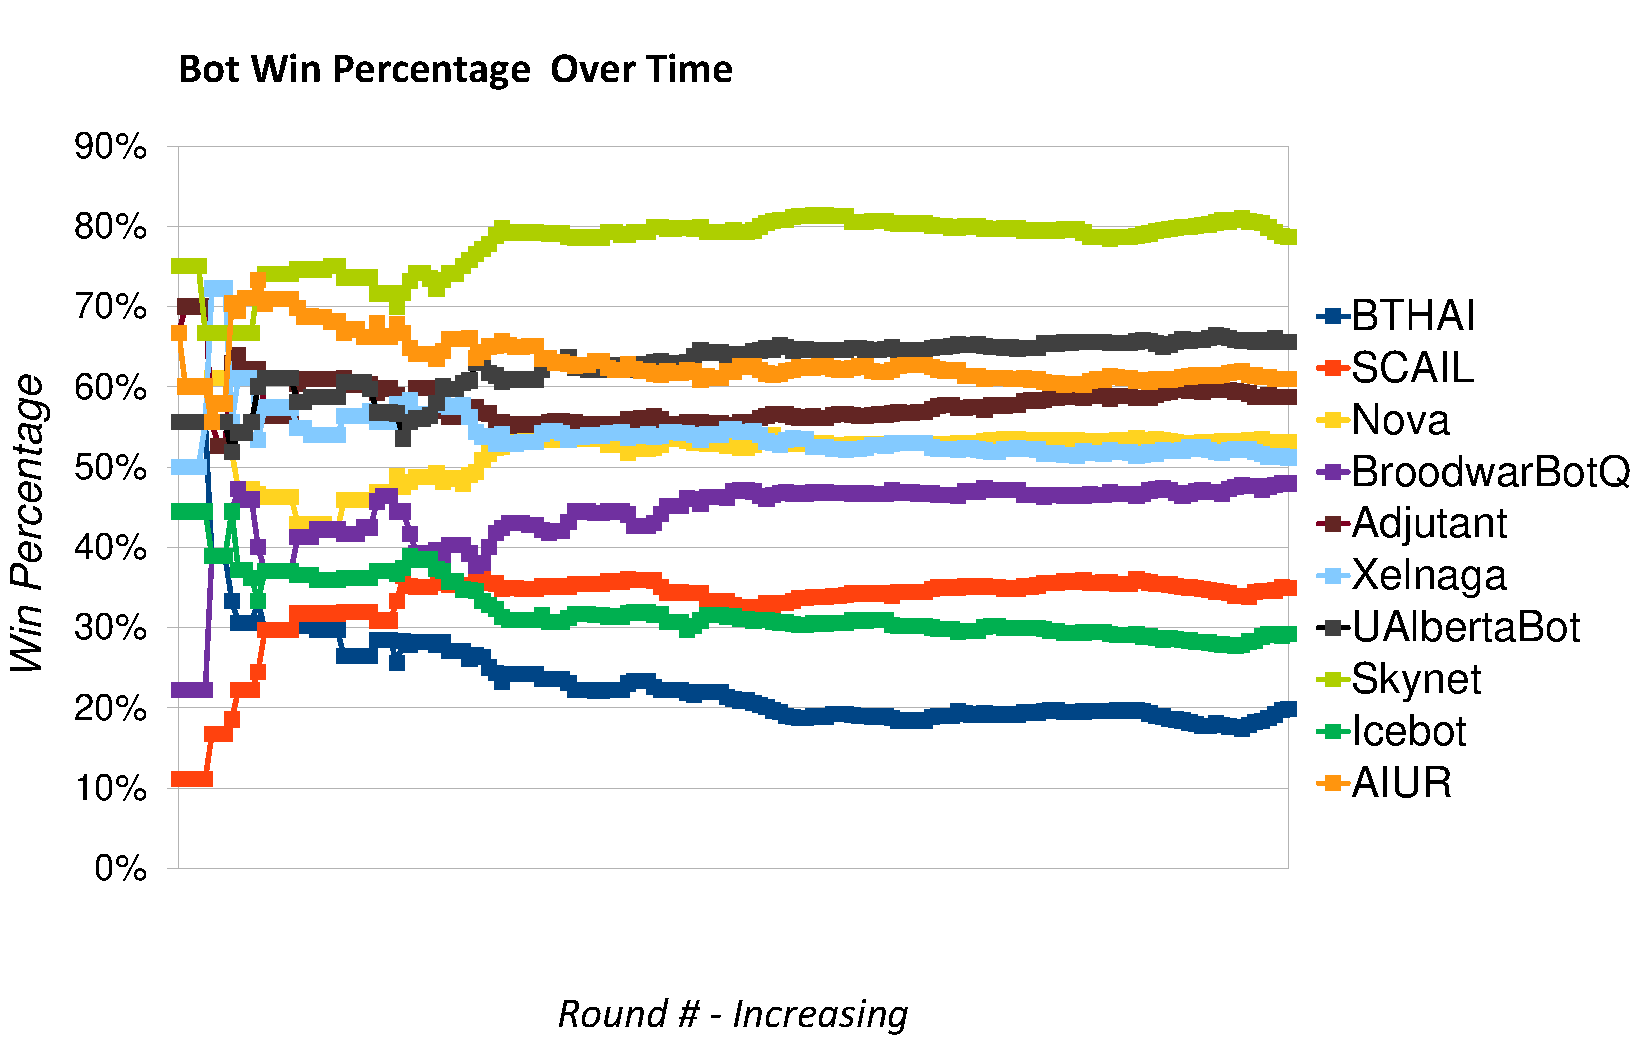
\includegraphics[width=\columnwidth]{figures/cig2012-ResultsRound90.pdf}
	%\vspace*{-1ex}
    \caption{Evolution of the win percentage of each bot participating in the
CIG 2012 competition}
    \label{fig:cig2012-results}
\end{figure}

\begin{figure*}[b]
	%\vspace*{-2ex}
    \centering
    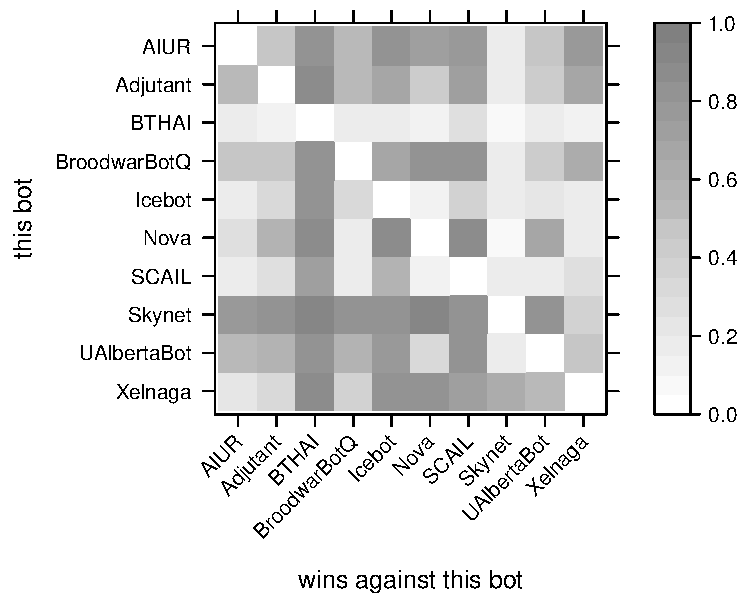
\includegraphics[width=0.32\textwidth]{figures/vstable3.pdf}
    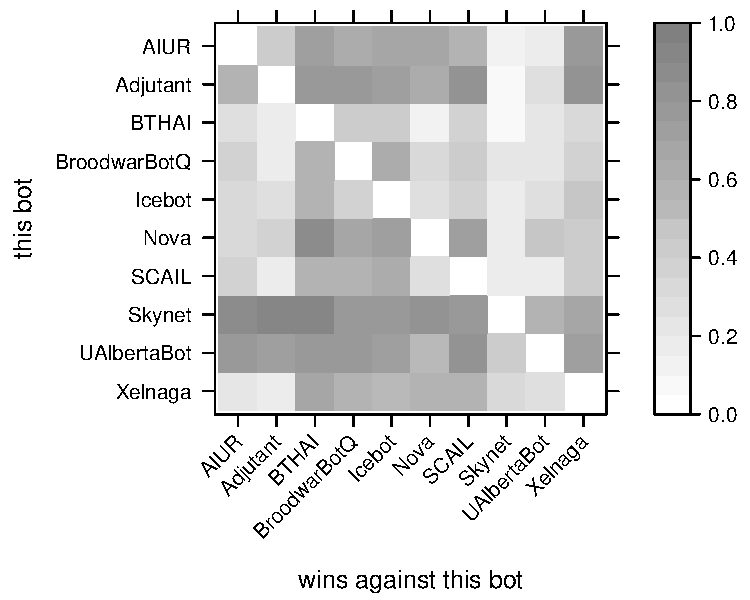
\includegraphics[width=0.32\textwidth]{figures/vstable6.pdf}
    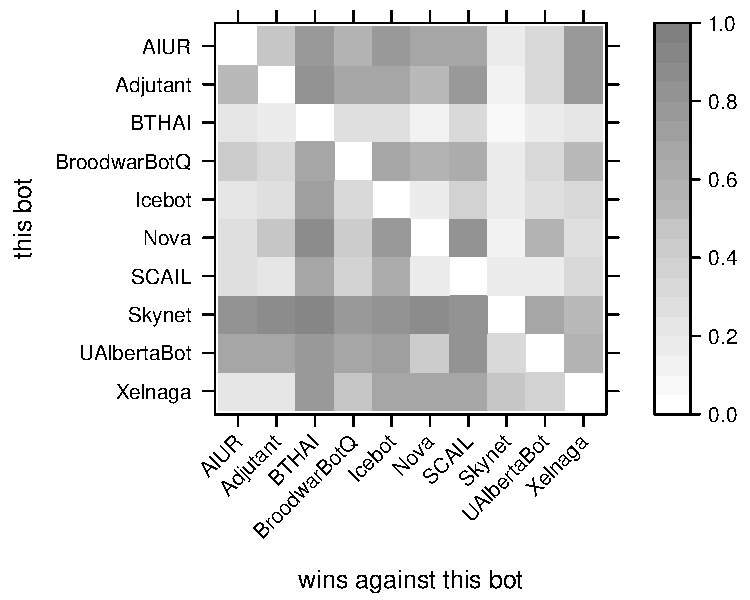
\includegraphics[width=0.32\textwidth]{figures/vstable.pdf}
	%\vspace*{-4ex}
    \caption{Win percentages of CIG 2012 competition, from left
    to right: 3-player maps only, 6-player maps only, all maps.
    Read from line to column, bot in row wins given fraction of
    games against bot in column. For some bots, we find interesting
    differences, e.g. Xelnaga gets worse on 6-player maps, UAlbertaBot
    gets better. Only Xelnaga can reliably beat Skynet, but only on 
    3-player maps}
    \label{fig:cig2012-mapresults}
\end{figure*}

As the CIG competition games were executed manually due to
a lack of available software (the AIIDE program was not yet
available at that time), the organizers separated the ten entries into
two brackets. In each bracket of 5 bots, a round-robin
tournament was held with 10 repetitions per pairing, resulting
in 40 games per bot.
The 5 maps chosen for the first round were selected from the pool
of well-known league play maps found on the Internet:
\emph{(2)MatchPoint 1.3}, \emph{(4)Fighting Spirit 1.3}, 
\emph{iCCup Destination 1.1}, \emph{iCCup Gaia}, and 
\emph{iCCup Great Barrier Reef}. Each bot pairing played
on every map twice, with switched starting positions.


The two top bots of every bracket qualified
for the final round. Table~\ref{tab:cig-first-round} summarizes
the results.
Note that as BroodwarBotQ and BTHAI have the same number of wins,
their direct encounter was evaluated which accounted 6:4 for the BroodwarBotQ.
The bots going into the final were thus UAlbertaBot, Skynet (from bracket A)
and Xelnaga and BroodwarBotQ (from bracket B). All qualified bots play the
Protoss faction. Most bots proved pretty stable, only Xelnaga and Protoss 
Beast Jelly crashed relatively often (each in more than a quarter of the games). 
Crashing of course resulted in an instant win for the other bot.
In some cases, neither bot was able to finish the other off completely,
so that they went into a passive state. We manually ended such games after
around 15 minutes and assigned victory to the bot that had obtained more
points as indicated on the end game screen.

\begin{table}[!b]
\caption{Results of the CIG 2011 competition}
\label{tab:cig-final-round}
\centering
\begin{tabular}{|c|c|c|c|c|}
\hline
{\bfseries Rank} & {\bfseries Crashes} & {\bfseries Games} & {\bfseries Bot} & {\bfseries Win \%} \\
\hline
1 & 0 &  30 &  Skynet       &  86.7\%\\
2 & 0 &  30 &  UAlbertaBot  &  73.3\%\\
3 & 3 &  30 &  Xelnaga      &  36.7\%\\
4 & 2 &  30 &  BroodwarBotQ   &  3.3\%\\
\hline
\end{tabular}
\end{table}



\subsubsection{Final Round}
\label{sec:cig-final-round}

The final round was played in a similar mode as each of the
first round brackets,
using another set of 5 previously unknown maps:
\emph{iCCup lost temple 2.4}, \emph{iCCup rush hour 3.1},
\emph{iCCup swordinthemoon 2.1}, \emph{iCCup yellow 1.1},
and \emph{La\_Mancha 1.1}. 
Letting each pairing play on each map twice again with
switching starting positions resulted in 30 games per bot.
The final results are displayed in table~\ref{tab:cig-final-round},
indicating Skynet as winner and UAlbertaBot as runner-up, being
almost equally strong, and the two other bots as clearly inferior.
The competition setup, documentation and results can be found
in\footnote{\url{http://ls11-www.cs.tu-dortmund.de/rts-competition/StarCraft-cig2011}}.

\subsubsection{CIG 2012}

For CIG 2012, the AIIDE tournament software was employed,
leading to a total of $4050$ games played in $90$ rounds
of round robin. As 6 different maps were used, this means
that each bot played every other on every map 15 times. 
As in the AIIDE competition, writing to and reading from
a bot specific directory was enabled, however, due to 
technical reasons, this feature was constrained to the
computer (of 6) the game was actually run on. We can 
therefore assume that this feature was of minor use for
the CIG competition. The only other difference to the
AIIDE competition was that the used maps were not 
made available to the competitors in advance. 

These maps came in two flavors, namely three 3-player maps:
\emph{Athena-II}, \emph{Neo Moon Glaive}, \emph{Tears of the Moon},
and three 6-player maps:
\emph{Legacy}, \emph{River of Light}, and 
\emph{The Huntress 1.1}. 
We shall note that some bots consistently crashed on one
of the originally considered maps which has thus been replaced.
This is surprising as all maps are well known league play maps
or have been provided with the StarCraft Brood War distribution
itself.
Setup, replays and results for the CIG 2012 competition can be found
here\footnote{\url{http://ls11-www.cs.tu-dortmund.de/rts-competition/StarCraft-cig2012}}.

\begin{table}[t]
\caption{Results of the CIG 2012 competition.}
\label{tab:cig2012}
\centering
\begin{tabular}{|c|c|c|}
\hline
{\bfseries Rank} & {\bfseries Bot} & {\bfseries Win \%} \\
\hline
1 & Skynet & 78.3\% \\
2 & UAlbertaBot & 65.2\% \\
3 & AIUR & 60.4\% \\
4 & Adjutant & 58.6\% \\
5 & Nova & 52.4\% \\ 
\hline
\end{tabular}
\end{table}

% \begin{figure*}[tb]
%     \centering
%     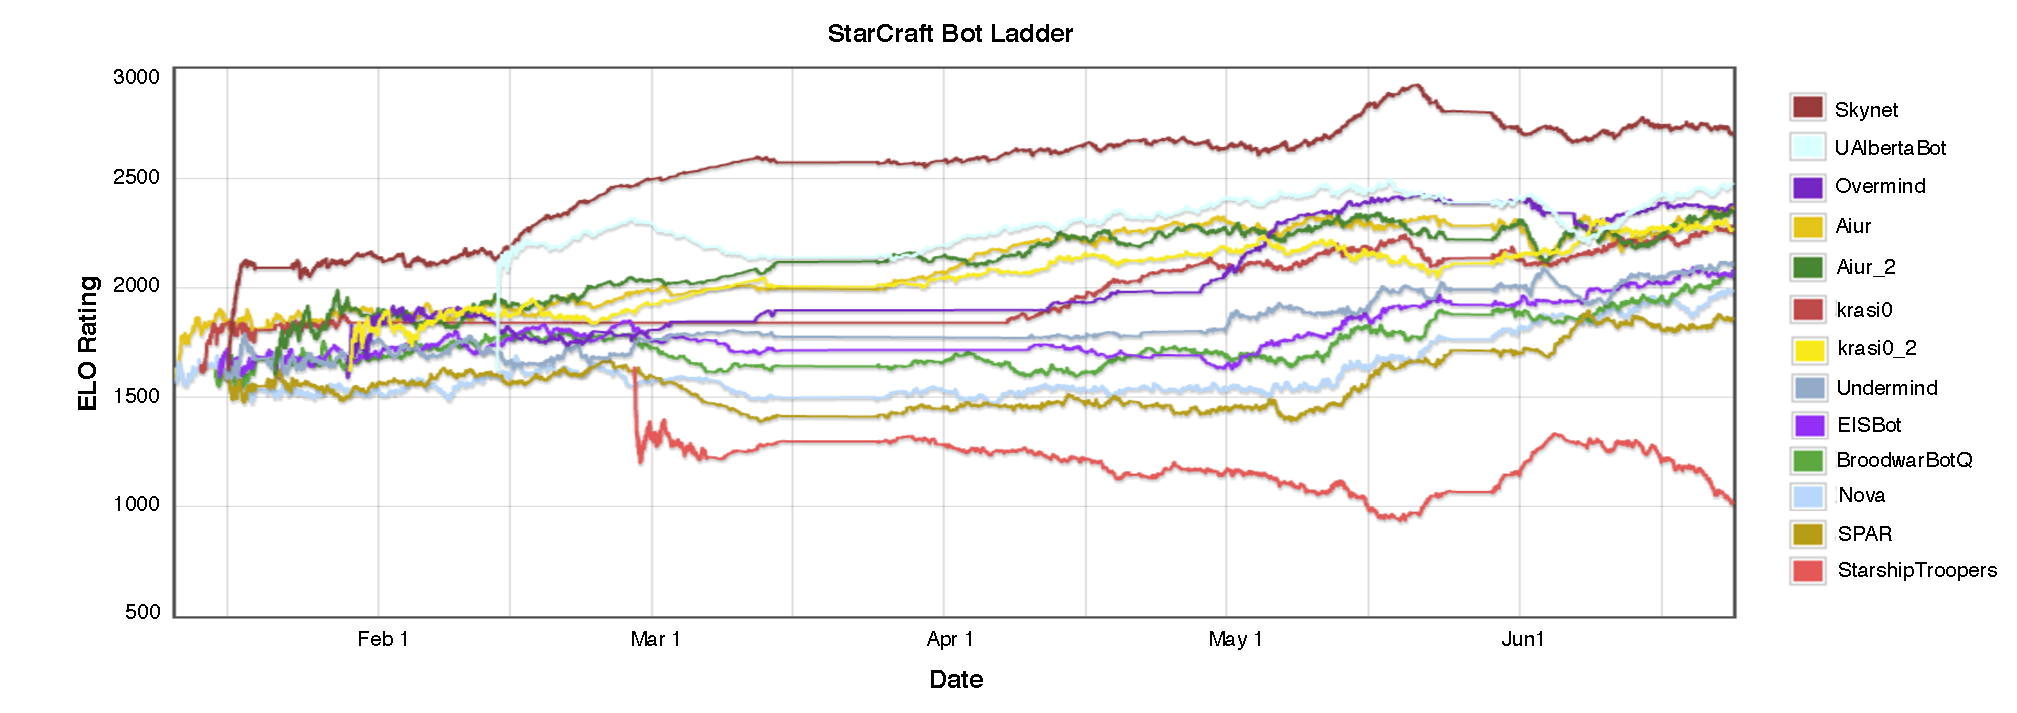
\includegraphics[width=\textwidth]{figures/botLadder1.pdf}
%     \caption{Bot's Elo Rating from February 1, 2012 to June 20, 2012}
%     \label{fig:botLadder1}
% \end{figure*}

% \begin{figure*}[tb]
%     \centering
%     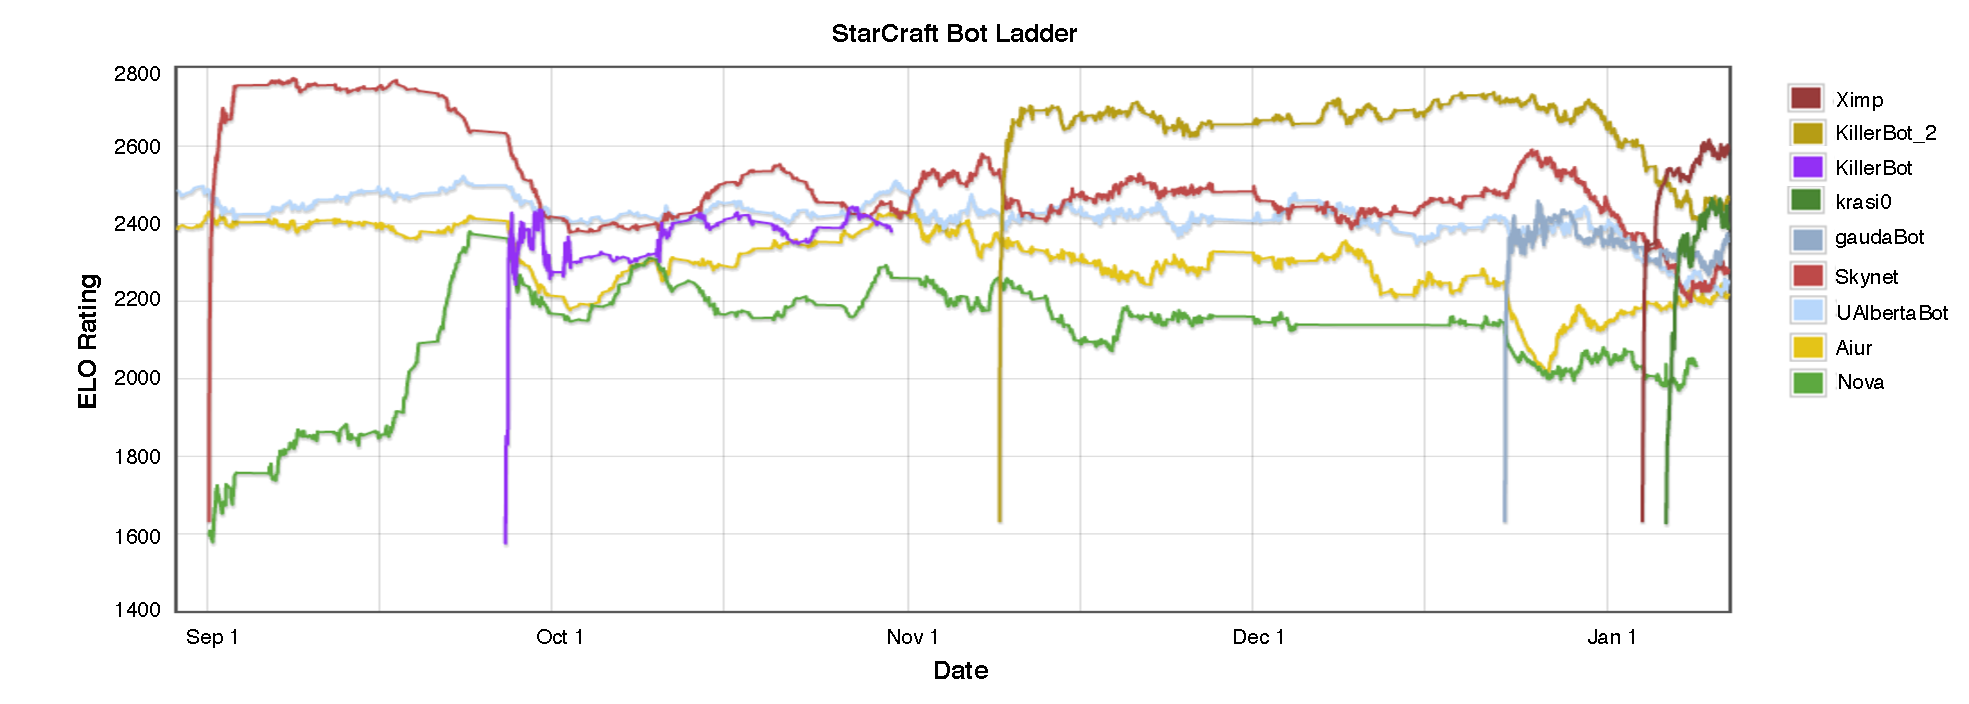
\includegraphics[width=\textwidth]{figures/botLadder2.pdf}
%     \caption{Bot's Elo Rating from September 1, 2012 to January 10, 2013}
%     \label{fig:botLadder2}
% \end{figure*}

The overall results are displayed in table~\ref{tab:cig2012},
and the win rate evolution over time in figure~\ref{fig:cig2012-results}.
These are quite consistent with the results of the AIIDE 2012 competition,
so that we can conclude that the best bots are not very dependent on 
knowing the maps beforehand. However, the bot vs. bot win rates as
displayed in figure~\ref{fig:cig2012-mapresults} show some interesting
trends. On the maps with more possible start points, some bots do 
better than others, namely SCAIL, Adjutant, Nova, and UAlbertaBot,
the latter probably due to its very efficient scouting routine.
Some bots however suffer from the increased uncertainty about
the enemies' position, namely Xelnaga and BroodwarBotQ.

As already observed before in the previously described competitions,
there are also bots who consistently beat top ranked bots but have
severe problems against lower ranked bots. E.g., Xelnaga is especially
strong against Skynet on the 3-player maps (about 70\% wins). Reviewing
the replays led to the assumption that Xelnaga usually tries to attack
Skynet's probes with a dark templar strategy, and often succeeds. 
Nova does very well against the UAlbertaBot, and the replays show
that it sometimes succeeds to lure the probes into its own base, where
they get killed, leading to severe resource problems. However, we cannot
tell how often this happens as this would require to review every single
replay between the 2 bots. Summarizing, most bots seem to have improved,
which becomes clear if the nearly unchanged BTHAI bot is taken as a baseline.
In 2011, it won more than half of its qualifying games, in 2012 it came
out last with around 20\% wins. However, designing a bot in order to 
beat a top bot (as for Xelnaga with Skynet) leads to a very restricted
strategy that often leads to failure if playing against different bots.
Note that in the direct encounter between Xelnaga and AIUR, its ancestor,
Xelnaga looses consistently.

Nevertheless, from the observations we made during the tournament,
we can draw the conclusion that the available bots are still 
very constrained. No bot in the competition played the Zerg race,
which is surprising as the AIIDE 2010 winner (Overmind) did so.
Presumably, implementing a good Zerg strategy is more demanding
than implementing one for the Protoss or Terran races. Many bots consistently crashed
when playing against a random race built-in bot for testing, and
also did so when the map size was changed from $128\times 128$ to 
any other. Furthermore, every single bot sometimes failed to finish
off an already beaten opponent, such that the game had to be stopped
after a previously determined maximum time. It also seems that most of
the current bots are not very good at adapting their strategy to the
one of their opponent during a game, or at least (via the read/write
procedure of game information) within a series of games.

\subsubsection{CIG 2013}

Mike will fill this out?

\begin{table}[t]
\caption{Results of the CIG 2013 competition.}
\label{tab:cig2013}
\centering
\begin{tabular}{|c|c|c|}
\hline
{\bfseries Rank} & {\bfseries Bot} & {\bfseries Win \%} \\
\hline
1 & Skynet & 91.1\% \\
2 & UAlbertaBot & 67.4\% \\
3 & AIUR & 54.9\% \\
4 & Xelnaga & 53.6\% \\
5 & Adjutant & 42.4\% \\ 
\hline
\end{tabular}
\end{table}

\subsubsection{CIG 2014}
The CIG 2014 competition was organized by Kyung-Joong Kim, Ho-Chul Cho, and In-Seok Oh of Sejong University. For 2014, the CIG competition used a total of 20 different maps which were unknown to the competitors before the competition started, which was by far the most maps ever used in a Starcraft AI competition and presented a challenge to many of the bots who entered. A total of 4680 games were played which meant that each bot played each other bot 60 times, or 3 times per map. The CIG 2014 competition was held just a few weeks before the AIIDE 2014 competition and so many of the entrants to the competition were identical, and the results definitely showed this. The top 4 bots were all the same as the 2014 AIIDE competition with IceBot coming 1st, Ximp in 2nd, LetaBot in 3rd and Aiur in 4th place. For descriptions of these bots please refer to the AIIDE 2014 competition description as none of the top-finishing bots had any significant changes made.

\begin{table}[t]
\caption{Results of the CIG 2014 competition.}
\label{tab:cig2014}
\centering
\begin{tabular}{|c|c|c|}
\hline
{\bfseries Rank} & {\bfseries Bot} & {\bfseries Win \%} \\
\hline
1 & IceBot & 83.1\% \\
2 & Ximp & 78.1\% \\
3 & LetaBot & 68.5\% \\
4 & Aiur & 66.1\% \\
5 & UAlbertaBot & 60.0\% \\ 
\hline
\end{tabular}
\end{table}


\subsubsection{CIG 2015}
There were some significant rule changes to the CIG 2015 competition, which was once organized by mebers from Sejong University. The most significant rule change was that entrants no longer had to be open source, in an attempt to attract more competitors who may not want to open source their bots. The second rule change was that a single competitor could submit multiple entries to the competition - which caused some controversy among registrants since this introduces the possibility of collusion between entries. Thankfully no such collusion was detected during the competition. The 2015 competition was also not run quite as long as previous competitions with only 2730 games being played in total, or 30 between each bot pairing, 6 between each bot on each of the 5 chosen maps. There were several new Zerg entries to the CIG 2015 competition which ended up finishing in the top three positions, with results very similar to those of the AIIDE 2015 competition. ZZZBot took 1st place, tscmoo-Z (a Zerg bot written by tscmoo) came 2nd, and Overkill came 3rd. For descriptions of these bots and their strategies used please refer to the AIIDE 2015 competition section as the strategies remained largely unchanged between the CIG and AIIDE competitions. 

\begin{table}[t]
\caption{Results of the CIG 2015 competition.}
\label{tab:cig2015}
\centering
\begin{tabular}{|c|c|c|}
\hline
{\bfseries Rank} & {\bfseries Bot} & {\bfseries Win \%} \\
\hline
1 & ZZZBot & 81.03\% \\
2 & tscmoo-Z & 73.59\% \\
3 & Overkill & 62.05\% \\
4 & LetaBot & 61.54\% \\
5 & Ximp & 60.26\% \\ 
\hline
\end{tabular}
\end{table}

% \subsection{StarCraft Bot Ladder}\label{sec:ladder}

% The StarCraft Bot Ladder is a website\footnote{\url{http://bots-stats.krasi0.com}} where bot versus bot matches are automatized, and are running all the time. This ladder is a great resource for creating data sets (all the game replays are available) and statistics. For bot ranking, the ladder uses an Elo rating system suitable for calculating the \emph{relative skill level} of a bot in two-player games. In the Elo system each player has a numerical rating that gets incremented or decremented some points after each game. The amount of points depends on the difference in the ratings of the players. A player will gain more points by beating a higher-rated player than by beating a lower-rated player. This kind of rating system is widely used in games like chess. This bot ladder compiles different versions of bots from the main worldwide competitions (like AIIDE, CIG or SSCAI\footnote{\url{http://sscaitournament.com}}), even some independent or ``under construction'' bots. Therefore, it is a very good resource to test the performance of new bots against the current state of the art in StarCraft bots before participating in the official competitions.

% Figure \ref{fig:botLadder1} shows the Elo rating of the bots in the ladder during the first half year of 2012. The ranking is practically equal than the AIIDE 2011 competition, showing the lack of adaptability of the current bots. We can notice these more extremely in Figure \ref{fig:botLadder2} for the second half year of 2012. During this period new bots were introduced in the ladder. We can observe how the first version of KillerBot made a huge impact on Skynet ranking and finally, the second version of KillerBot quickly became the best bot for more than one month (again we can see how the rest of the bots aren't able to adapt and the ranking doesn't change so much). And finally, in January, the Ximp bot appears with a new strategy that overcomes the rest of the bots. Both KillerBot and Ximp use hard-coded strategies without any kind of adaptation capabilities. However, they implement strategies that no other bot has a counter for, and thus manage to win a very large percentage of games. This points out, once again, that one of the major open challenges in RTS game AI is how achieving adaptive strategies, that can recognize the opponent's intentions, and select an adequate response.


% \subsection{Adaptation Analysis}

% One of the major conclusions from the results of the StarCraft competitions is the lack of adaptation of bots.  Some switch between different build-orders, but do not fully adapt their strategy. No bot is capable of observing the opponent and autonomously synthesize a good plan from scratch to counter the opponent strategy. In this section we analyzed this claim quantitatively using the tools of \cite{SynnaeveOpeningCig11}. We analyzed the replays from the 2011 and 2012 AIIDE competitions (shown in Figures \ref{fig:aiide2011-botopenings} and \ref{fig:aiide2012-botopenings} respectively). We analyzed the way bots choose their openings depending on which other bot they are playing against. Given that there is no dominant strategy in StarCraft, and that it is necessary to see what the opponent is doing in order to determine the best opening, we would expect bots to change their openings depending on which other bot they are playing (since each bot uses a different strategy, or set of strategies). Using clustering, we identified the most common openings in all the replays from the 2011 and 2012 competitions (each one shown with a different color in the figures). No data is shown for the ItayUnvermind bot, since its opening did not match significantly with any of the ones used in our study (extracted from humans pro-gamers).

% \begin{figure*}[tb]
%     \centering
%     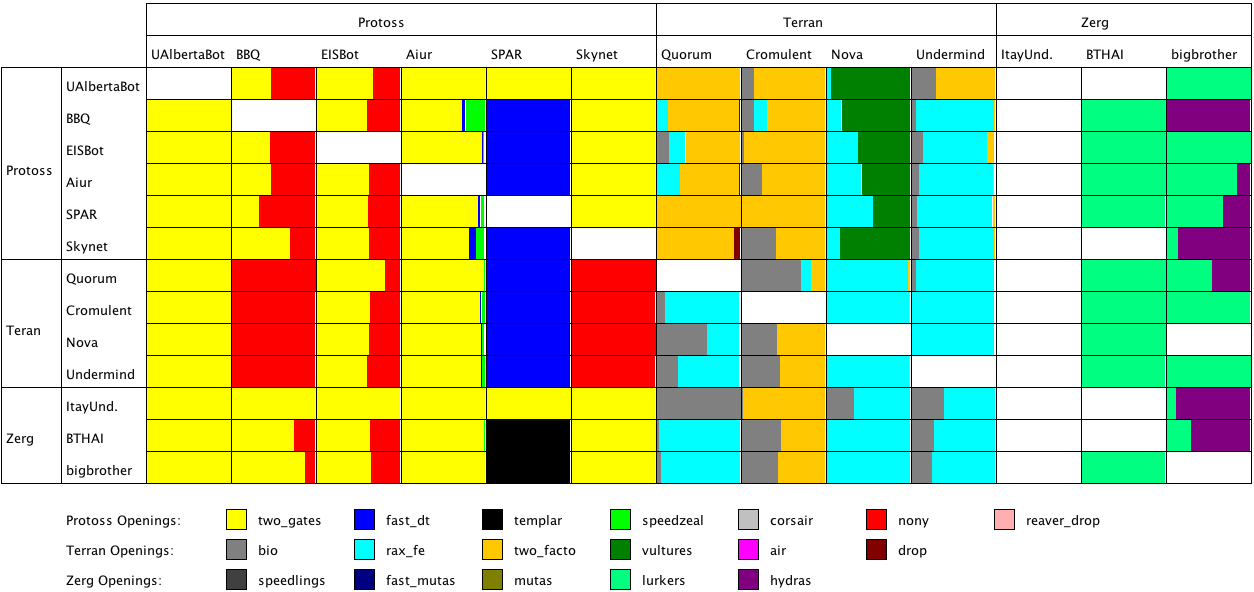
\includegraphics[width=\textwidth]{figures/botopenings2011.png}
%     \caption{Distribution of different openings performed by the different bots participating in the AIIDE 2011 competition. For each bot match-up, the colors show the proportion of times that the column bot used a particular opening against the row bot.}
%     \label{fig:aiide2011-botopenings}
% \end{figure*}

% \begin{figure*}[tb]
%     \centering
%     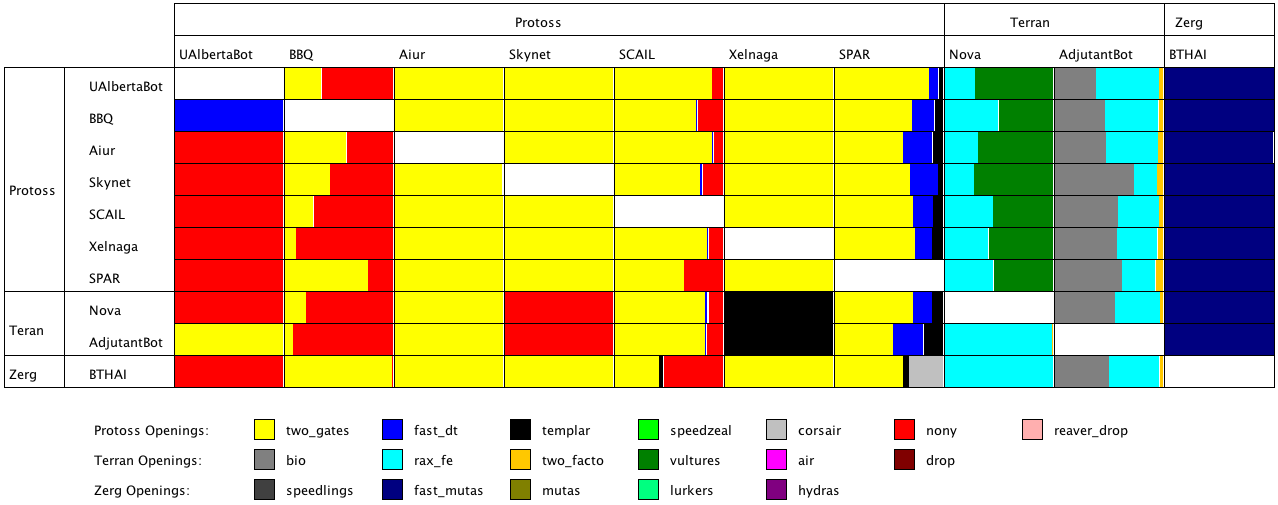
\includegraphics[width=\textwidth]{figures/botopenings2012.png}
%     \caption{Distribution of different openings performed by the different bots participating in the AIIDE 2012 competition. For each bot match-up, the colors show the proportion of times that the column bot used a particular opening against the row bot.}
%     \label{fig:aiide2012-botopenings}
% \end{figure*}

% Specifically, we identified the following openings (for a better comprehension of strategies, buildings or units of StarCraft, we refer the reader to Teamliquid's wiki\footnote{\url{http://wiki.teamliquid.net/starcraft/Category:Strategies}}):
% \begin{itemize}
%   \item Protoss openings:
%   \begin{itemize}
%     \item \emph{two\_gates}: Build two \emph{Gateways} and keep training \emph{Zealots} (basic contact attack ground unit), this is the quickest way to apply pressure.
%     \item \emph{fast\_dt}: Produce \emph{Dark Templars} (technologically advanced stealth ground unit) as soon as possible, sacrificing early game power for a technological advance, hard-countered by detectors technology.
%     \item \emph{templar}: Train \emph{High Templars} (technologically advanced zone attack unit) as fast as possible, same as above, less deadly but is less easily countered.
%     \item \emph{speedzeal}: Train \emph{Zealots} and research attack and speed upgrades as soon as possible, some early game power transitioning into late game tech.
%     \item \emph{corsair}: Produce \emph{Corsairs} (air-air flying unit) as soon as possible and then transition into training \emph{Dark Templars} (safe from Zerg's flying detectors thanks to \emph{Corsairs}), \emph{Reavers} (ground artillery unit) or \emph{Dragoons}. Weak early game.
%     \item \emph{nony}: Build three \emph{Gateways} and massive training of \emph{Dragoons}. Slower than \emph{two\_gates} but still some early game (ranged) power.
%     \item \emph{reaver\_drop}: Train \emph{Reavers} as soon as possible to be able to do drops (air transport of artillery units).
%   \end{itemize}
%   \item Terran openings:
%   \begin{itemize}
%     \item \emph{bio}: Produce a large army of \emph{Marines} (basic ranged ground unit) and \emph{Medics} (can heal biological units). Quickest way to apply pressure.
%     \item \emph{rax\_fe}: Take the closest ``natural expansion'' as soon as possible. This provides a big economic boost in the mid game by sacrificing some early game power.
%     \item \emph{two\_facto}: Build two \emph{Factories} and keep producing \emph{Tanks} (ground artillery unit). Vulnerable while building up to it and then very powerful on ground.
%     \item \emph{vultures}: Produce mainly \emph{Vultures} (fast ground ranged unit, excels against small units) and research mines. Quicker to reach (technologically) and build than tanks, can transition into tanks.
%     \item \emph{air}: Produce \emph{Wraiths} (ranged flying units) as soon as possible for an air attack. Vulnerable to anti-air openings or quick rushes.
%     \item \emph{drop}: Train \emph{Dropships} (flying transports) as soon as possible to be able to do (mostly tanks or marines) drops, leveraging efficient tactics.
%   \end{itemize}
%   \item Zerg openings:
%   \begin{itemize}
%     \item \emph{speedlings}: Train \emph{Zerlings} (basic cheap, fast, ground contact attack unit) and research speed upgrade as soon as possible. Quickest way to apply pressure.
%     \item \emph{fast\_mutas}: Produce mainly \emph{Mutalisks} (ranged flying units). Vulnerable in the early game while gathering gas and researching the technology.
%     \item \emph{mutas}: Expand two times for a stronger economy before massive training of \emph{Mutalisks}. Slower but more powerful build-up than above.
%     \item \emph{lurkers}: Train \emph{Lurkers} (ground, stealth artillery unit) as soon as possible to benefit from their (advanced technology) zone attack and cloak ability. 
%     \item \emph{hydras}: Massive production of \emph{Hydralisks} (ground ranged unit). Much quicker to reach technologically than \emph{Lurkers} and can transition into them.
%   \end{itemize}
% \end{itemize}

% As the figures show, the top three ranked bots in the competition (Skynet, Aiur and UalbertaBot) do not change their strategy at all depending on their opponent. For example, the Skynet bot (both in 2011 and 2012), always uses the same opening (\emph{two\_gates}), except when playing a Terran opponent, when it uses \emph{nony}. This reflects the trend that the performance of bots is still more dependent on carefully handcrafted and non-adaptive behaviors, than on on-line decision making procedures. This is so, since most of the problems that need to be solved in order to implement such procedures are still open.


% {\color{blue} to-do}

\bibliographystyle{splncs}
\bibliography{references}

\end{document}



